
\begin{SCfigure*}
	\centering
	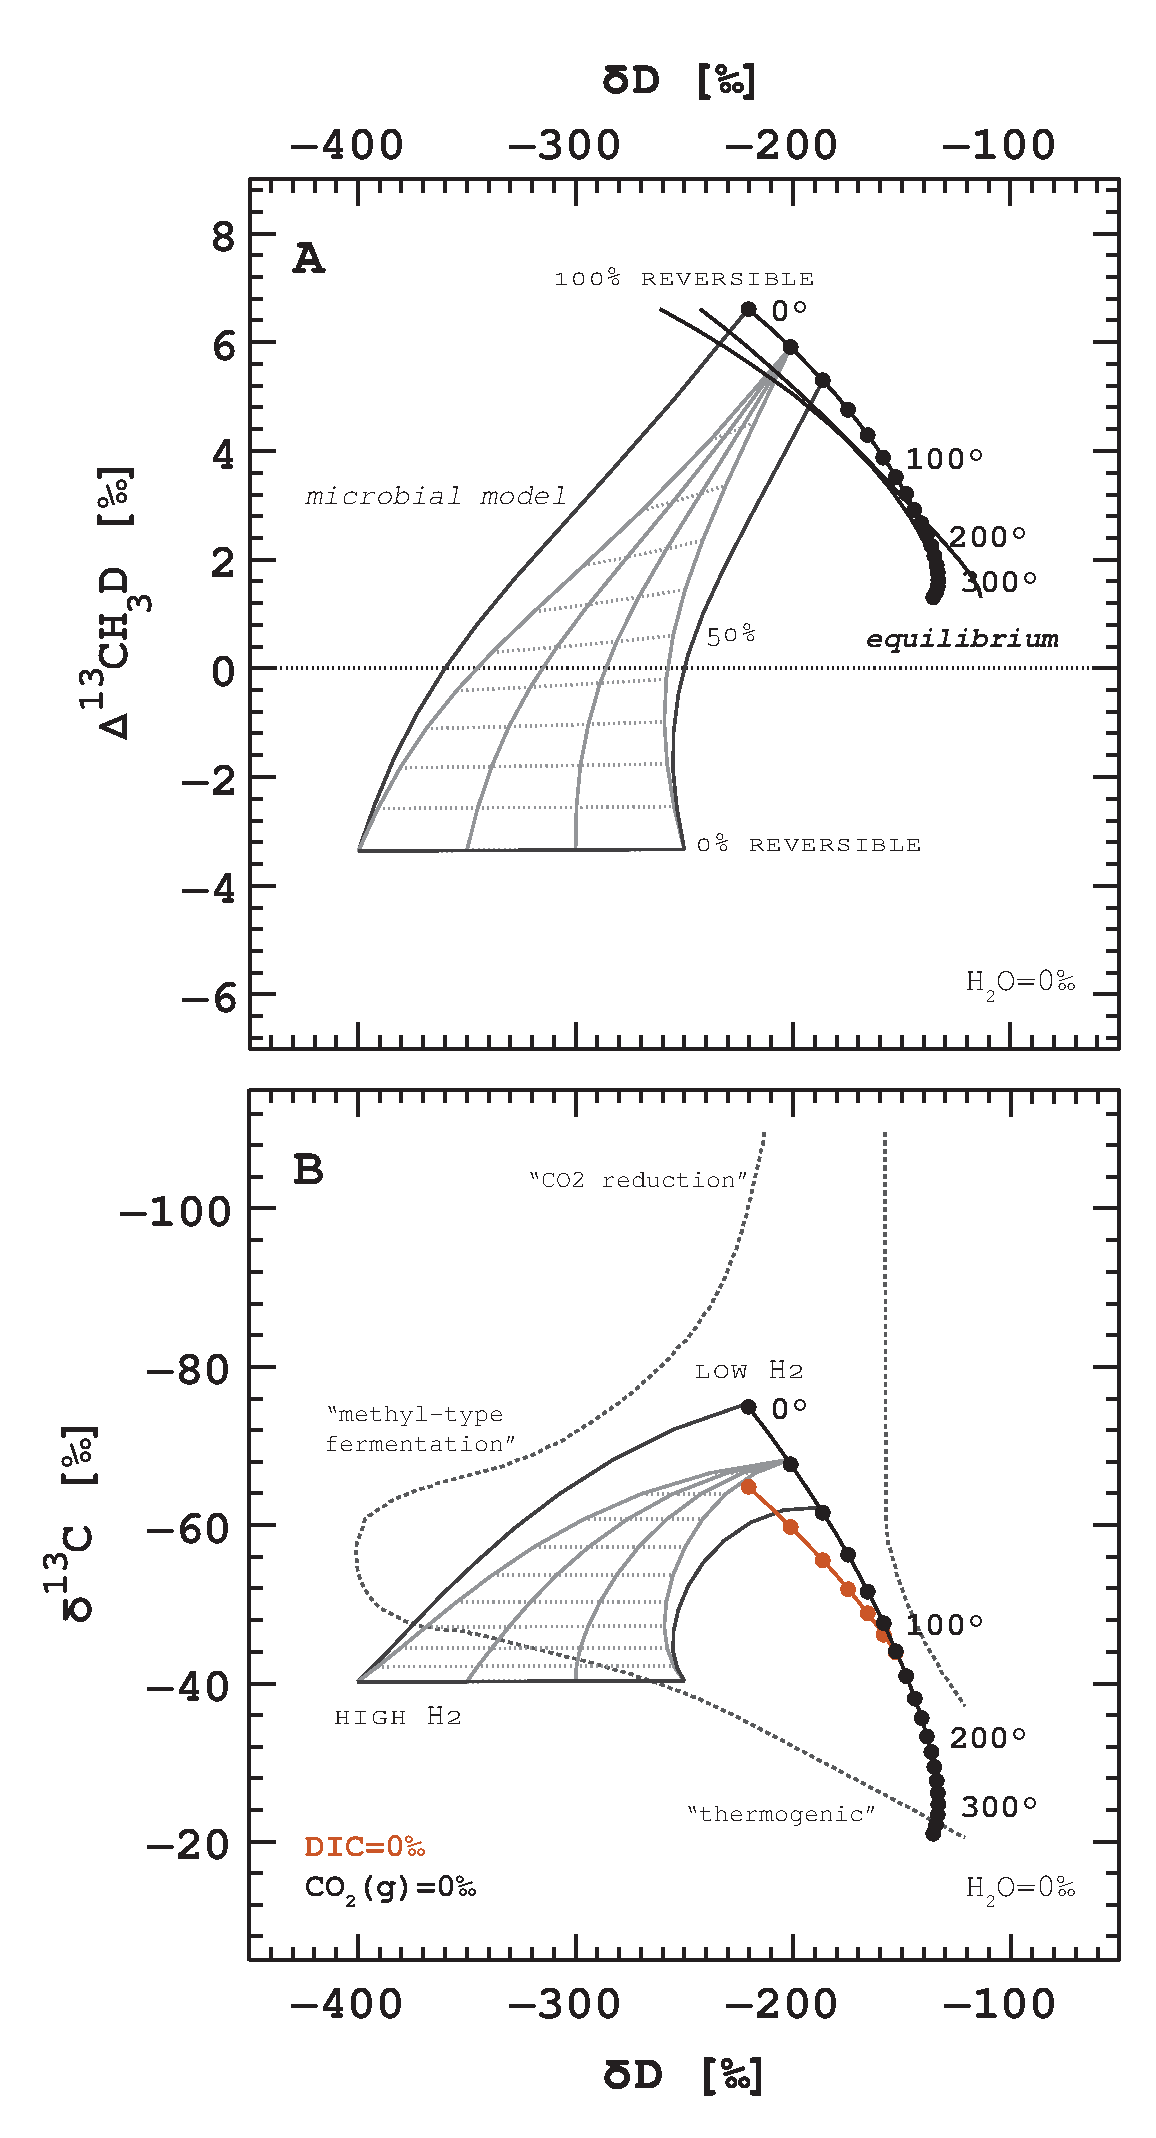
\includegraphics[scale=0.42]{figures/Fig5.4.pdf}
%	\captionsetup{format=myregular}	% no hrule beneath caption
	\caption[Predicted ratios of CH\textsubscript{4} isotopologues
	produced during hydrogenotrophic methanogenesis]{Model of isotopologue abundances in CH\textsubscript{4}
		produced during microbial methanogenesis from
		CO\textsubscript{2}+H\textsubscript{2} \parencite{Wang++_2015_S}. The model
		trajectories begin from a fully-reversible (equilibrium) line whose
		position is determined by assuming δ\textsuperscript{13}C of DIC or
		CO\textsubscript{2} are 0‰ vs.\ PDB. (This assumption is easily changed
		if, for example CO\textsubscript{2} has a higher
		\textsuperscript{13}C/\textsuperscript{12}C ratio than PDB.) The
		underlay in (B) is the outline of the frequently-used plot from \textcite{Whiticar_1990_OG}.
		
		\quad The plot indicates that modeled isotopic compositions for the
		fully-kinetic endmember are enriched in \textsuperscript{13}C and
		depleted in D relative to the equilibrium endmember. The fully-kinetic
		endmember is related to high H\textsubscript{2} concentrations (which
		yield a very large (negative) Δ\textsubscript{r}\emph{G}) \parencite{Burke_1993_Chemosphere}.
		Therefore, hydrogenotrophic methanogens could produce
		CH\textsubscript{4} with isotopic signatures indistinguishable from
		those typically attributed to methylotrophic or acetoclastic
		methanogenesis \parencite{Whiticar_1990_OG,Vinson++_2017_CG}. Whether this is
		true will require evaluation by experiments under low H\textsubscript{2}
		conditions \parencite{Valentine++_2004_GCA,Kawagucci++_2014_GCA,Okumura++_2016_ProgEPS} or \emph{in vitro} \parencite{Scheller++_2013_JACS_KIE}. Caveats to this
		model include (\emph{i}) the assumed fractionation factors may not
		approximate reality well, and (\emph{ii}) the possibility that the
		H-addition steps involved in methanogenesis may be differentially
		reversible in nature.}
	\label{fig:5:4}
\end{SCfigure*}
